\documentclass{article}
\usepackage[landscape]{geometry}
% \usepackage{pdflscape}
\usepackage{fancyhdr}
\usepackage{multicol}
\usepackage[english]{babel}
\usepackage[utf8]{inputenc}
\usepackage[T1]{fontenc}
\usepackage{lmodern}
\usepackage{amsmath}
\usepackage{amssymb}
\usepackage{amsthm}
\usepackage{float}
\usepackage{array}
\usepackage{booktabs}
\usepackage{color}
\usepackage{listings}
\usepackage[explicit]{titlesec}
\usepackage{tikz}
\usepackage{enumitem}
\usepackage{ifthen}
\usepackage[unicode]{hyperref}
\hypersetup{
	colorlinks,
	citecolor=black,
	filecolor=black,
	linkcolor=black,
	urlcolor=black
}

\geometry{left = 2cm, right = 0.75cm, top = 2cm, bottom = 0cm}

\pagestyle{fancy}
\fancyhf{}
\lhead{Team Dolores TUMbridge (TU München)}
\chead{\sectionName}
\rhead{\thepage}
\setlength{\headsep}{3pt}

\setlist[itemize,1]{leftmargin=12pt} % Horizontal indentation in itemize environment
\setlength{\tabcolsep}{4pt} % Horizontal indentation between table columns
\setlength{\columnsep}{5pt} % Horizontal indentation between page columns

\newcounter{seccnt}
\newcounter{subseccnt}[seccnt]
\newcounter{subsubseccnt}[subseccnt]


\setcounter{tocdepth}{3}
\setcounter{secnumdepth}{3}

\setlist{nosep}

\makeatletter
\renewcommand\tableofcontents{%
	\@starttoc{toc}%
}
\makeatother

\definecolor{blue}{rgb}{0,0.4,1}
\definecolor{green}{rgb}{0.4,0.7,0}
\definecolor{orange}{rgb}{0.8,0.5,0}

\titleformat{\section}
{{\color{green}\hrule\hrule\hrule\hrule\hrule\hrule}\vskip-.1ex\normalfont\large\bfseries}
{\setlength{\fboxrule}{2pt}\fcolorbox{green}{green}{\makebox[.83cm][c]{\textcolor{white}{\thesection}}}\hspace{.3em}}
{0pt}
{#1}
\titlespacing{\section}{0pt}{0ex}{0ex}

\titleformat{\subsection}
{\normalfont\normalsize\bfseries}
{\setlength{\fboxrule}{2pt}\fcolorbox{green}{white}{\makebox[.83cm][c]{\thesubsection}}\hspace{.3em}}
{0pt}
{#1}
\titlespacing{\subsection}{0pt}{0ex}{0ex}

\titleformat{\subsubsection}
{\normalfont\normalsize\bfseries}
{\setlength{\fboxrule}{1pt}\fcolorbox{green}{white}{\makebox[.9cm][c]{\thesubsubsection}}\hspace{.3em}}
{0pt}
{#1}
\titlespacing{\subsubsection}{0pt}{0ex}{0ex}

\lstdefinestyle{custom}{
	tabsize=2,
	showspaces=false,
	showstringspaces=false,
%	breakatwhitespace=true,
	breaklines=true,
	basicstyle=\footnotesize\ttfamily,
	keywordstyle=\color{blue},
	commentstyle=\color{green},
	stringstyle=\color{orange},
}

\lstset{style=custom}


\newcommand{\sectionPath}{}
\newcommand{\subsectionPath}{}
\newcommand{\subsubsectionPath}{}
\newcommand{\sectionName}{}
\newcommand{\subsectionName}{}
\newcommand{\subsubsectionName}{}

\newcommand{\setSection}[2][\sectionPathName]{
	\def\sectionPathName{#2}
	\noindent\begin{minipage}{\linewidth}
		\section{#2}\label{sec:#1}
	\end{minipage}
	\stepcounter{seccnt}
	\renewcommand{\sectionPath}{#1/}
	\renewcommand{\subsectionPath}{}
	\renewcommand{\subsubsectionPath}{}
	\renewcommand{\sectionName}{#2}
}

\newcommand{\setSubsection}[2][\subsectionPathName]{
	\def\subsectionPathName{#2}
	\subsection{#2}\label{sec:#1}
	\stepcounter{subseccnt}
	\renewcommand{\subsectionPath}{#1/}
	\renewcommand{\subsubsectionPath}{}
}


\newcommand{\setSubsubsection}[2][\subsubsectionPathName]{
	\def\subsubsectionPathName{#2}
	\subsubsection{#2}\label{sec:#1}
	\stepcounter{subsubseccnt}
	\renewcommand{\subsubsectionPath}{#1/}
}

\newif\ifcodeexpected
\newif\ifcodeislatex

\newcommand{\sssloadCode}[2]{
	\def\loadCodePath{Algorithms/#2#1}
	\IfFileExists{Algorithms/#2#1}{
		\ifcodeislatex
			\input{Algorithms/#2#1}
		\else
			\IfFileExists{Algorithms/#2overview.tex}{
				\input{Algorithms/#2overview.tex}
			}{}
			\lstinputlisting{Algorithms/#2#1}
		\fi
		\codeexpectedfalse
	}{}
}

\newcommand{\ssloadCode}[2]{
	\ifthenelse{\equal{\subsubsectionPath}{}}{
		\sssloadCode{#1}{#2}
	}{
		\sssloadCode{#1}{#2\subsubsectionPath}
		\ifcodeexpected\sssloadCode{#1}{#2\arabic{subsubseccnt}\subsubsectionPath}\fi
	}
}

\newcommand{\sloadCode}[2]{
	\ifthenelse{\equal{\subsectionPath}{}}{
		\ssloadCode{#1}{#2}
	}{
		\ssloadCode{#1}{#2\subsectionPath}
		\ifcodeexpected\ssloadCode{#1}{#2\arabic{subseccnt}\subsectionPath}\fi
	}
}

\newcommand{\loadCode}[1][code.cpp]{
	\codeexpectedtrue
	\ifthenelse{\equal{\sectionPath}{}}{
		\sloadCode{#1}{}
	}{
		\sloadCode{#1}{\sectionPath}
		\ifcodeexpected\sloadCode{#1}{\thesection\sectionPath}\fi
	}
	\ifcodeexpected	{\bf\color{red}{Error: \sectionPath\subsectionPath\subsubsectionPath#1 not found!\\}}\fi
}

\newcommand{\loadContent}[1][content.tex]{
\codeislatextrue
\loadCode[#1]
\codeislatexfalse
}



\title{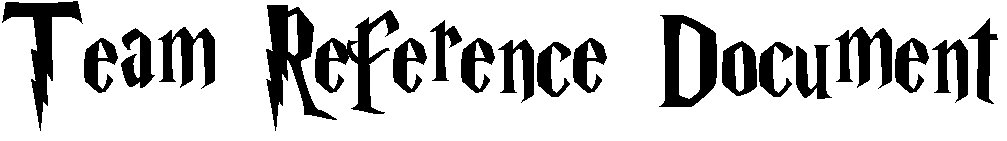
\includegraphics[width=0.9\columnwidth]{heading.png}}
\author{Team Dolores TUMbridge -- TU München}
\date{}

\begin{document}
	% \begin{landscape}
		\footnotesize
		\begin{multicols}{3}

			\maketitle

			\thispagestyle{fancy}

			\tableofcontents
			%\columnbreak

			\setSection{General}

			\lstset{language=bash}

			\setSubsection{Compilation}
			\loadCode[script.sh]

	%		\setSubsection{Running}
	%		\loadCode[script.sh]
			\stepcounter{subseccnt}

			\setSubsection{Debugging}
			\loadCode[script.sh]

			\lstset{language=C++}

		%	\setSubsection{Code}
		%	\loadCode[program.cpp]
			\stepcounter{subseccnt}

			% \setSubsection[InputOutput]{Input and Output}
			% \loadCode
			\stepcounter{subseccnt}

			% \setSubsection{VIM}
			% \loadCode[vimrc.vimrc]
			\stepcounter{subseccnt}

			\setSubsection{Random}
			\loadCode

			\setSubsection[LanguageSpecificFunctionalities]{Language Specific Functionalities}
			\loadCode

			\setSection[DynamicProgramming]{Dynamic Programming}

			\setSubsection[LongestIncreasingSubsequence]{Longest Increasing Subsequence}
			\loadCode

			\setSubsection[DivideAndConquerOptimization]{Divide and Conquer Optimization}
			\loadCode

			\setSubsection[KnuthsOptimization]{Knuths Optimization}
			\loadCode
			
			\setSubsection[AlienTrick]{Alien Trick}
			\loadCode

			\setSubsection[Knapsack]{Knapsack}
			\loadCode

			\setSection{Graphs}
			\subsection{Theorems}

\subsubsection{Euler’s theorem}
For any planar graph, $V - E + F = 1 + C$, where $V$ is the number of graph's vertices, $E$ is the number of edges, $F$ is the number of faces in graph's planar drawing, and $C$ is the number of connected components. Corollary: $V-E+F=2$ for a 3D polyhedron.

\subsubsection{Vertex covers and independent sets}
Let $M, C, I$ be a max matching, a min vertex cover, and a max independent set. Then $|M| \le |C| = N -|I|$, with equality for bipartite graphs. Complement of an MVC is always a MIS, and vice versa. Given a bipartite graph with partitions $(A,B)$, build a network: connect source to $A$, and $B$ to sink with edges of capacities, equal to the corresponding nodes' weights, or 1 in the unweighted case. Set capacities of the original graph's edges to the infinity.
Let $(S, T)$ be a minimum $s-t$ cut. Then a maximum(-weighted) independent set is $I = (A \cap S)\cup(B \cap T)$,
and a minimum(-weighted) vertex cover is $C = (A - T) \cup (B \cap S)$.

\subsubsection{Erd\H{o}s Gallai: Degree Sequence}
A sequence $d_1 \geq d_2\dots \geq d_n$ is a degree sequence of a simple graph if and only if $\sum_{i = 1}^{n}d_i$ is even and $ \sum_{i = 1}^{k}d_i \leq k\left(k - 1\right) +  \sum_{i = k + 1}^{n} \min \left\{d_i, k\right\}$ holds for all $1 \leq k \leq n$.

\subsubsection{Cayley's formula (Prüfer sequence)}
\noindent\textbf{Theorem:} There are exactly $n^{n - 2}$ trees on $n$ labelled vertices.

\noindent\textbf{Prüfer sequence:} Bijection between labelled trees of size $n$ and sequences of length $n - 2$.
\begin{itemize}
	\item \textit{Tree to sequence}: For $n - 2$ times, remove the leaf with smallest label and add its neighbour to the sequence.
	\item \textit{Sequence to tree}: From left to right, until the sequence is empty, connect the first element from the sequence $v$ to the lowest-label element $u$ that is unmarked and not in the sequence. Mark $u$ and remove $v$ from the sequence. In the end, connect the two remaining unmarked vertices.
	\item Note that vertex $v$ appears $\operatorname{deg}\left(v\right) -1$ times in the sequence.
\end{itemize}
\noindent\textbf{Similar results:}
\begin{itemize}
	\item The number of spanning trees of a labelled complete bipartite graph $U \cup V$ is $\left|U\right|^{\left|V\right| - 1} \cdot \left|V\right|^{\left|U\right| - 1}$.
	\item The number of labelled rooted forests on $n$ vertices is $\left(n + 1\right)^{n - 1}$ (simply add one virtual vertex).
	\item The number of labelled forests with $k$ connected components such that $1, \dots, k$ all belong to different components is $kn^{n - k - 1}$. % See Takacs, Lajos (March 1990). "On Cayley's formula for counting forests". Journal of Combinatorial Theory, Series A. 53 (2): 321–323. doi:10.1016/0097-3165(90)90064-4
\end{itemize}

			\setSubsection{Traversal}

			\setSubsubsection[ArticulationPointsBridges]{Articulation Points Bridges}
			\loadCode

			\setSubsubsection[StronglyConnectedComponents]{Strongly Connected Components}
			\loadCode

			\setSubsection{Matching}

			\setSubsubsection[BipartiteMatching]{Max Cardinality Bipartite Matching}
			\loadCode

			\setSubsubsection[BipartiteVertexCover]{Min Bipartite Vertex Cover}
			\loadCode

			\setSubsubsection[MinCostMatching]{Min Cost Bipartite Matching}
			\loadCode

			\setSubsubsection[GeneralMatching]{General Matching}
			\loadCode

			% \setSubsubsection[Hafnian]{Hafnian}
			% \loadCode

			\setSubsection{Flow}

			\setSubsubsection[MaximumFlowPushRelabel]{Max Flow -- Push Relabel}
			\loadCode

			\setSubsubsection[MaxFlowDinic]{Max Flow Dinic}
			\loadCode

			\setSubsubsection[MinimumCostMaximumFlow]{Min Cost Max Flow}
			\loadCode

			\setSubsubsection[MinimumCostMaximumFlowCapacityScaling]{Min Cost Max Flow Capacity Scaling}
			\loadCode

			\setSubsection[LowestCommonAncestor]{Lowest Common Ancestor}
			\loadCode

			\setSubsection[EdgeColoring]{Edge Coloring}
			\loadCode

			\setSubsection[CentroidDecomposition]{Centroid Decomposition}
			\loadCode

			\setSection[DataStructures]{Data Structures}

			\setSubsection[UnionFindDisjointSets]{Union Find Disjoint Sets}
			\loadCode

			\setSubsection[SparseTable]{Sparse Table}
			\loadCode

			\setSubsection[FenwickTree]{Fenwick Tree}
			\loadCode

			\setSubsection[Data]{Data}
			\loadCode

			\setSubsection[SegmentTree]{Segment Tree}
			\loadCode

			\setSubsection[PersistentSegmentTree]{Persistent Segment Tree}
			\loadCode

			\setSubsection[LinkCutTree]{Link Cut Tree}
			\loadCode

			\setSubsection[ConvexHullTrick]{Convex Hull Trick}

			\setSubsubsection[PartiallyDynamicConvexHullTrick]{Partially Dynamic}
			\loadCode

			\setSubsubsection[DynamicConvexHullTrick]{Dynamic}
			\loadCode

			\setSubsubsection[LiChaoSegmentTree]{Li Chao Segment Tree}
			\loadCode

			\setSubsection{Treap}

			\setSubsubsection{BST}
			\loadCode

			%\setSubsubsection{Implicit}
			%\loadCode

			%\setSubsubsection{Persistent}
			%\loadCode

			\setSubsection[OrderStatisticsTree]{Order Statistics Tree}
			\loadCode[program.cpp]

			\setSubsection[HeavyLight]{Heavy Light Decomposition}
			\loadCode

			% \setSubsection[PermutationTree]{Permutation Tree}
			% \loadCode

			\setSubsection[Queuetrick]{Queue-like undoing}
			\loadCode

			\setSection{Strings}

			\setSubsection{Basics}
			\loadCode

		%	\setSubsection[StringHashing]{String Hashing}
		%	\loadCode

			\setSubsection{Trie}
			\loadCode

			\setSubsection[SuffixArray]{Suffix Array}
			\loadCode

			\setSubsection[StringMatching]{String Matching (KMP)}
			\loadCode

			\setSubsection[ZAlgorithm]{Z-Algorithm}
			\loadCode

		%	\setSubsection[StringAlignment]{String Alignment}
		%	\loadCode

			\setSubsection[LongestPalindrome]{Longest Palindrome}
			\loadCode

			\setSubsection[Eertree]{Eertree}
			\loadCode

			\setSubsection[SuffixAutomaton]{Suffix Automaton}
			\loadCode

			\setSubsection[AhoCorasick]{Aho-Corasick}
			\loadCode

			\setSection{Geometry}

			\setSubsection[2DGeometry]{2D Geometry}
			\loadCode

			\setSubsection[NearestPairOfPoints]{Nearest pair of points}
			\loadCode

			\setSubsection[HalfPlaneIntersection]{Half-plane Intersection}
			\loadCode

			\setSubsection[3DGeometry]{3D Geometry}
			\loadContent

			\setSubsubsection[SphericalDistance]{Spherical Distance}
			\loadCode

			\setSubsubsection[3DPoint]{Point}
			\loadCode

			\setSubsubsection[3DConvexHull]{Convex Hull}
			\loadCode

			\setSubsubsection[PolyhedronVolume]{Volume of Polyhedron}
			\loadCode


			\setSection{Mathematics}

			\setSubsection{Theorems}


	%		\setSubsubsection{Fast exponentiation}

	%		\begin{itemize}
	%			\item $x^{n}=\begin{cases}
	%			x&\text{if }n=1\\{(x^{\frac{n}{2}})}^{2}&\text{if }2\mid n\\x^{n-1}*x&\text{otherwise}
	%			\end{cases}$
	%		\end{itemize}

			\setSubsubsection{Fibonacci numbers}

			\begin{itemize}
				\item Definition:
				\begin{itemize}
					\item $f_{0}=0,\ f_{1} = 1,\ f_{i} = f_{i-1}+f_{i-2}$
				\end{itemize}
				\item Calculation:
				\begin{itemize}
					\item Dynamic programming: $O(n)$
					\item Fast matrix exponentiation: $O(\log{n})$
					\item $\begin{bmatrix}1&1\\1&0\end{bmatrix}^{n}=\begin{bmatrix}f_{n+1}&f_{n}\\f_{n}&f_{n-1}\end{bmatrix}$
				\end{itemize}
				\item $\sum\limits_{k=0}^n \binom{n-k}{k} = F_{n+1}$
				\item Generating function $f(z) = \frac{1}{1-z-z^2}$
			\end{itemize}

			\setSubsubsection{Series Formulas}
			\def\arraystretch{1.4}
			\noindent\begin{tabular}{ll}
				$\sum\limits_{k=0}^n k=\frac{n(n+1)}{2}$&$\sum\limits_{k=0}^n k^4=\frac{6n^5+15n^4+10n^3-n}{30}$	\\
				$\sum\limits_{k=a}^b k=\frac{(a+b)(b-a+1)}{2}$ &	$\sum\limits_{k=0}^n k^5=\frac{2n^6+6n^5+5n^4-n^2}{12}$\\
				$\sum\limits_{k=0}^n k^2=\frac{n(n+1)(2n+1)}{6}$&$\sum\limits_{k=0}^n x^k=\frac{x^{n+1}-1}{x-1}$	\\
				$\sum\limits_{k=0}^n k^3=\frac{n^2(n+1)^2}{4}$&$\sum\limits_{k=0}^n kx^k=\frac{x-(n+1)x^{n+1}+nx^{n+2}}{(x-1)^2}$
			\end{tabular}

			\noindent\textbf{Geometric series:}
			\begin{itemize}
				\item $\sum_{i = 0}^{n}c^i = \frac{c^{n + 1} - 1}{c - 1}$ for $c \neq 1$
				\item  $\sum_{i = 0}^{ \infty }c^i = \frac{1}{1 - c}$ and $\sum_{i = 1}^{ \infty }c^i = \frac{c}{1 - c}$ for $\left|c\right| < 1$
			\end{itemize}

			\setSubsubsection{Binomial coefficients}

			\begin{itemize}
				\item Definition:
				\begin{itemize}
					\item $\binom{n}{k}=\frac{n!}{k!(n-k)!}$
					\item $\binom{n}{k}=\binom{n-1}{k-1}+\binom{n-1}{k}$
				\end{itemize}
			\end{itemize}
			\def\arraystretch{1.4}
			\noindent\begin{tabular}{ll}
				$\sum\limits_{m=k}^n \binom{m}{k} = \binom{n+1}{k+1}$ & $\sum\limits_{k=0}^m \binom{n+k}{k} = \binom{n+m+1}{m}$	\\
				$\sum\limits_{k=0}^n \binom{n}{k}^2 = \binom{2n}{n}$ & $\sum\limits_{k=1}^n k\binom{n}{k} = n2^{n-1}$ \\
				$\sum\limits_{k=1}^n k^2\binom{n}{k} = (n+n^2)2^{n-2}$ & $\sum\limits_{j=0}^k \binom{m}{j} \binom{n}{k-j} = \binom{n+m}{k}$ \\
				$\sum\limits_{m=0}^n \binom{m}{j} \binom{n-m}{k} = \binom{n+1}{k+j+1}$ &$\sum\limits_{j=0}^k (-1)^j \binom{n}{j} = (-1)^k \binom{n-1}{k}$ \\
				$\sum\limits_{k=q}^n \binom{n}{k} \binom{k}{q} = 2^{n-q} \binom{n}{q}$ & \\
				\multicolumn{2}{c}{$\sum\limits_{k=-a}^a (-1)^k \binom{a+b}{a+k}\binom{b+c}{b+k}\binom{c+a}{c+k} = \frac{(a+b+c)!}{a!b!c!}$}
			\end{tabular}
			\begin{itemize}
				\item There are exactly $\binom{\left|A\right| + \left|B\right|}{\left|A\right|}$ ways to select sets $A' \subseteq A$ and $B' \subseteq B$ such that $\left|A'\right| = \left|B'\right|$ (proof sketch: choose those not selected in $A$ and those selected in $B$): \newline
				$\sum\limits_{k=0}^{\min(n,m)} \binom{n}{k} \binom{m}{k} = \binom{n+m}{n}$
			\end{itemize}

			\setSubsubsection{Catalan's number}
			\begin{itemize}
				\item $1, 1, 2, 5, 14, 42, 132, 429, 1430, \dots$
				\item $c_n = \sum\limits_{k=0}^{n-1} c_k\,c_{n-1-k} = \frac{1}{n+1} \binom{2n}{n} = \binom{2n}{n}-\binom{2n}{n-1}$
				\item Number of correct bracket sequences consisting of $n$ opening and $n$ closing brackets.
				\item Generating function $f(x) = \frac{1-\sqrt{1-4x}}{2x}$
			\end{itemize}


			\setSubsubsection{Pentagonal Number theorem}
			\begin{itemize}
				\item $\prod_n (1-x^n) = \sum_k(-1)^kx^{k(3k-1)/2}$
				\item $\sum_np(n)x^n = \prod_n (1-x^n)^{-1}$ where $p$ is the partition function.
			\end{itemize}

			\setSubsubsection{Hook Length formula}
			\begin{itemize}
				\item Number of Young diagrams (filling of the cells with integers from $\{1,\cdots,n\}$ without repetitions) with shape $\lambda = (\lambda_1\geq\cdots\geq\lambda_k)$ and $n = \sum_i\lambda_i$: $f^\lambda = \frac{n!}{\prod h_\lambda(i,j)}$ where $h_\lambda(i,j)$ is the hook length of cell $(i,j)$. (number of cells below / right)
			\end{itemize}

			\setSubsubsection{Pick's theorem}
			$I = A - B/2 + 1$, where $A$ is the area of a lattice polygon, $I$ is number of lattice points inside it, and $B$ is number of lattice points on the boundary. Number of lattice points minus one on a line segment from $(0, 0)$ and $(x, y)$ is $gcd(x, y)$.

			\setSubsubsection{Burnside's Lemma}
			\begin{itemize}
				\item $ClassesCount = \frac{1}{|G|} \sum_{g \in G} |X^g|$
				\item $G$: group of operations(invariant permutations)
				\item $X^g$: set of fixed points for operation $g$, i.e. $X^g = \{x \in X: g.x=x \}$
				\item special case: $ClassesCount = \frac{1}{|G|} \sum_{g \in G} k^{c(g)}$
				\item $k$: "number of colors"
				\item $c(g)$: number of cycles in permutation
			\end{itemize}

			\setSubsubsection{Multinomial coefficients}
			$(x_1+...+x_m)^n = \sum\limits_{k_1+...+k_m=n, k_i \geq 0} \binom{n}{k_1,...,k_m} x_1^{k_1}...x_m^{k_m}$, where $\binom{n}{k_1,...,k_m} = \frac{n!}{k_1! k_2! ... k_m!}$ \newline
			in combinatorial sense $\binom{n}{k_1,...,k_m}$ is equal to the number of ways of depositing $n$ distinct objects into $m$ distinct bins, with $k_1$ objects in the first bin, $k_2$ objects in the second bin ...

			\setSubsubsection{Gray's code}
			direct: $G(n) = n \oplus (n>>1)$ \newline
			recurrent: $G(n) = 0G(n-1) \cup 1G(n-1)^R$ and $G(n)^R = 1G(n-1) \cup 0G(n-1)^R$

			\setSubsection{Game theory}

			\setSubsubsection{Grundy's function}
			For all transitions $v -> v_i$ compute the Grundy's function $f(v_i)$: \newline
			1. $v -> v_i$ transtion into one game, then compute $f(v_i)$ recursively \newline
			$v -> v_i$ transition into sum of several games, compute $f$ for each game and take $\oplus$ sum of their values \newline
			2. $f(v) = mex\{f(v_1),...,f(v_k)\}$ ($mex$ returns minimal number not contained in the set)

			\setSubsection[2SAT]{2-SAT}
			\loadCode

			\setSubsection[PointsUnderLine]{Lattice Points below a line}
			\loadCode

			\setSubsection[PrimeNumbers]{Prime numbers}
			\loadCode

			\setSubsection[PrimeFundamentals]{Algebra Basics}
			\loadCode

			\setSubsection[ModularInverse]{Modular Inverse}
			\loadCode

			\setSubsection[EulerTotient]{Euler's Totient Function and Theorem}
			\loadCode

			\setSubsection[DiscreteLogarithm]{Discrete Logarithm: Baby Gigant}
			\loadCode

			\setSubsection[DiscreteRoot]{Discrete Root}
			\loadCode

			\setSubsection[PrimitiveRoot]{Primitive Root (Generator)}
			\loadCode

			\setSubsection[RabinMiller]{Rabin Miller}
			\loadCode

			\setSubsection[PollardRho]{Pollard Rho}
			\loadCode

			\setSubsection[FFT]{Fast Fourier Transformation}

		%	\setSubsubsection[FFTRecursive]{Recursive Fast Fourier Transformation}
		%	\loadCode

			\setSubsubsection[FFTNonRecursive]{Non-Recursive Fast Fourier Transformation}
			\loadCode

			\setSubsubsection[NumberTheoreticTransform]{Number Theoretic Transform}
			\loadCode

			\setSubsubsection[MultipointEvaluation]{Multipoint Evaluation}
			\loadCode
			
			\setSubsubsection[Newton]{Newton Iteration}
			\loadCode

			\setSubsubsection[InverseSeries]{Inverse Series}
			\loadCode
			
			\setSubsubsection[PolynomialDivision]{Polynom Division with remainder}
			\loadCode

      \setSubsubsection[FWHT]{Fast Walsh-Hadamard transform}
      \loadCode
      
      \setSubsubsection[SubsetConv]{Subset convolution}
      \loadCode

			\setSubsection[LinearAlgebra]{Linear Algebra}

			\setSubsubsection[GaussJordan]{Gauss-Jordan}
			\loadCode

			\setSubsubsection[CharPoly]{Characteristic Polynomial}
			\loadCode

			\setSubsection[LinearRecurrence]{Linear Recurrence}
			\setSubsubsection[kth-term]{kth Term}
			\loadCode
			\setSubsubsection[BerlekampMassey]{Berlekamp-Massey}
			\loadCode

			\setSubsection[Simplex]{Simplex}
			\loadCode

		\end{multicols}
%		\clearpage\null\clearpage
	% \end{landscape}

\end{document}
